\documentclass{report}

\title{Mécatro: Rapport d'automatique}
\author{Groupe 7: Royer Jules, Simon Noah-Luc, Colin Matthieu, Bourderioux Armand}

\date{}

\usepackage[T1]{fontenc}
\usepackage{lmodern}

\usepackage[margin=0.7in]{geometry}

\usepackage{amssymb}
\usepackage{gensymb}
\usepackage{mathrsfs}

\usepackage{amsmath}
\usepackage{mathtools}

\usepackage{graphicx}
\usepackage{float}

\usepackage[parfill]{parskip}

\preto{\subsection}{\Needspace{5\baselineskip}}
\preto{\section}{\Needspace{5\baselineskip}}

\hyphenpenalty=10000

\usepackage{listings}
\usepackage{pxfonts}

\usepackage{biblatex}
\addbibresource{bibliography.bib}

\usepackage{blindtext}

\begin{document}

\maketitle

\tableofcontents

\chapter{Introduction}
Le but de la partie automatique du projet de mécatronique est de créer un contrôleur
pour un robot "bolide" suiveur de ligne. Le contrôleur a d'abord été créé théoriquement
dans le logiciel Matlab et testé sur un modèle de simulation Simulink, puis il a été
implémenté informatiquement en Arduino afin d'être embarqué dans le robot.

\chapter{Création du contrôleur théorique}

Contrôle d'un mouvement rectiligne uniforme.

En reprenant les notations et la modélisation du document "Equations de la dynamique du Segway",
les équations de la dynamique sous forme d'état sont:

\begin{equation*}
    \begin{cases}
        \dot{p} = \dot{u} \\
        \dot{u} = \frac{1}{\beta}\big( \frac{1}{\rho}kI^{+} - m_bdv^2 \big) \\
        \dot{\psi} = v \\
        \dot{v} = \frac{1}{\gamma}\big( \frac{lk}{2\rho}I^{-} + m_bduv \big) \\
        \dot{I^{+}} = \frac{U^{+}}{L} - \frac{R}{L}I^{+} - \frac{2k}{L\rho}u \\
        \dot{I^{-}} = \frac{U^{-}}{L} - \frac{R}{L}I^{-} - \frac{kl}{L\rho}v \\
        \dot{y} = u\sin\psi \\
    \end{cases}
\end{equation*}

Les entrées sont $U^{+}$, $U^{-}$.

Les sorties mesurées sont:

\begin{equation*}
    \begin{cases}
        \phi^{+} = \phi_{right} + \phi_{left} = \frac{2}{\rho}p \\
        \phi^{-} = \phi_{right} + \phi_{left} = \frac{l}{\rho}\psi \\
        c_{LF} = \frac{y}{\cos\psi} \approx y \\
    \end{cases}
\end{equation*}

Où on a défini:

\begin{itemize}
    \item $p$ la distance curviligne parcourue par le robot le long de sa trajectoire.
    \item $u$ sa vitesse longitudinale.
    \item $\psi$ l'angle entre l'axe horizontal $x$ et la direction du robot.
    \item $I^{-} = I_{right} - I_{left}$ la somme des courants des moteurs.
    \item $I^{-} = I_{right} - I_{left}$ la différence des courants.
    \item $U^{+} = U_{right} + U_{left}$ la somme des tensions aux bornes des moteurs.
    \item $U^{-} = U_{right} - U_{left}$ la différence des tensions.
    \item $\beta = M + \frac{2I^{\omega}_{y}}{\rho^2}$
    \item $\gamma = I_{\psi} + m_bd^2$
    \item $\phi^{+}$ la somme des angles des roues. Posons $\alpha = \frac{2}{\rho}$.
    \item $\phi^{-}$ la différence des angles des roues. Posons  $\eta = \frac{l}{\rho}$.
    \item $c_{LF}$ la mesure de l'écart entre le point A et la ligne (approximation en MRU horizontal).
\end{itemize}


\begin{figure}[h]  % Placement "here"
    \centering
    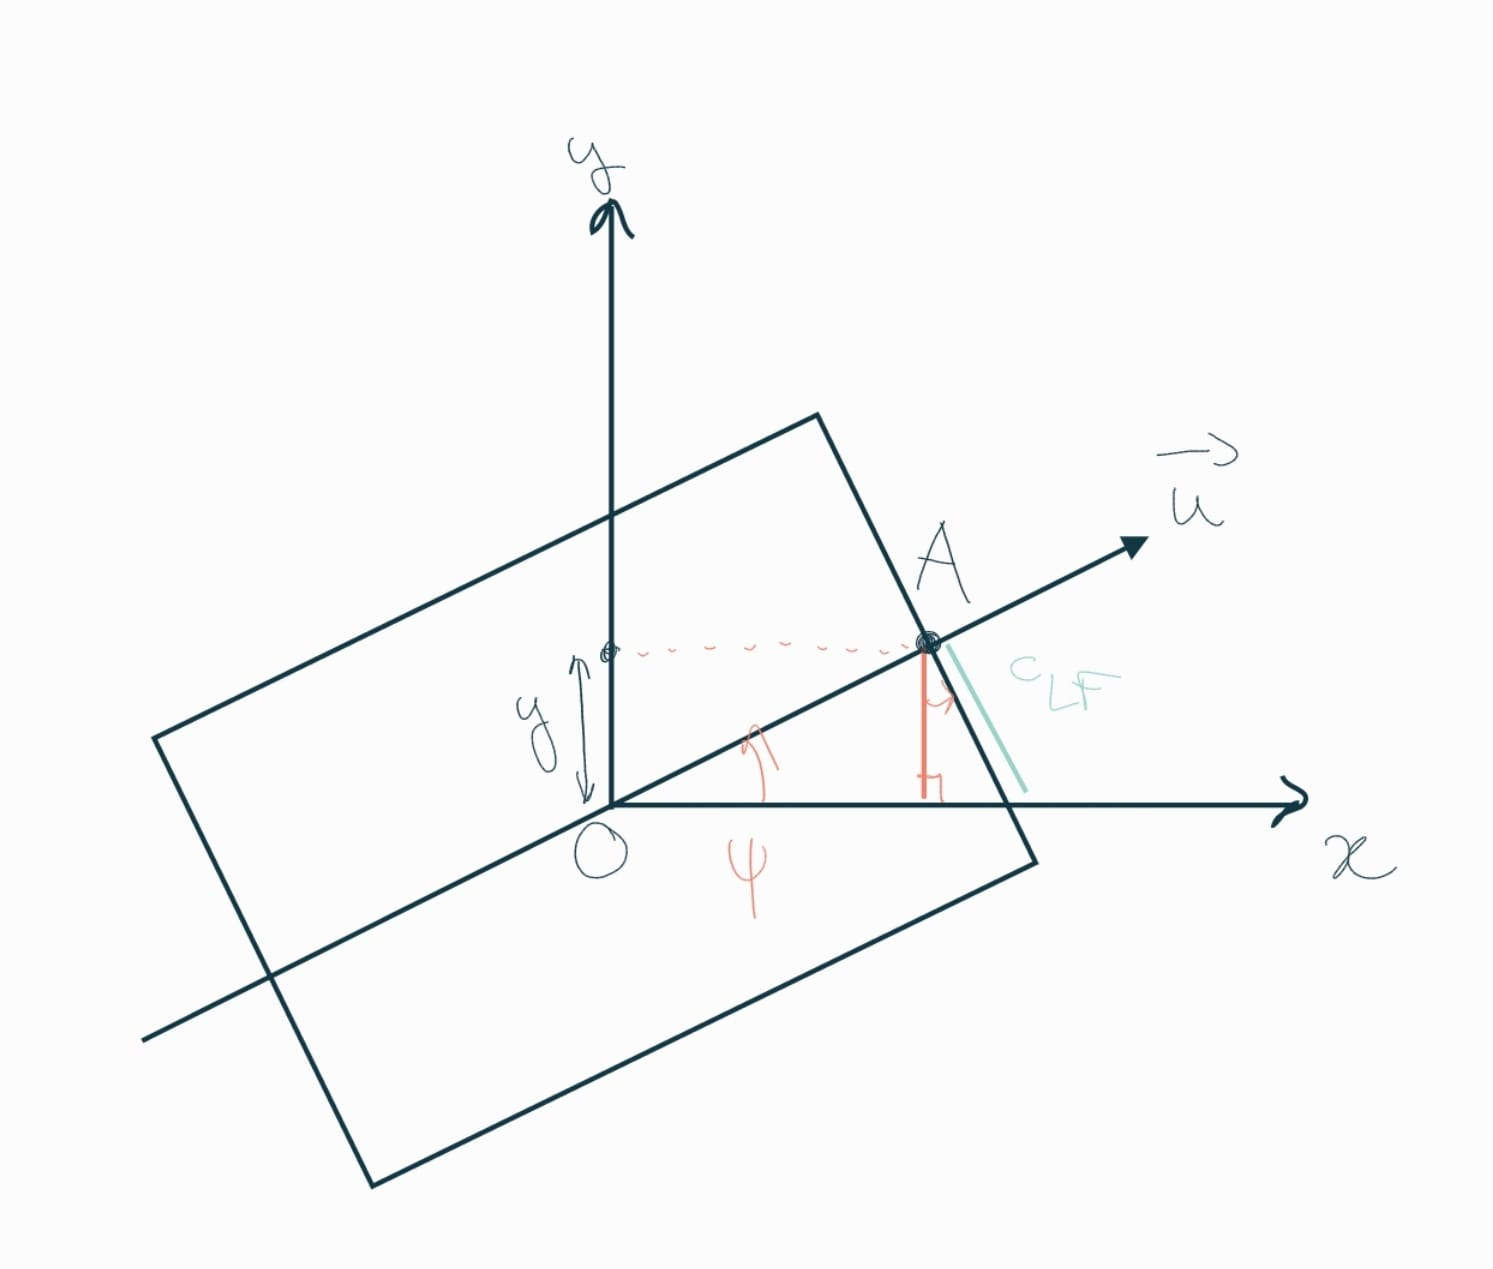
\includegraphics[width=0.5\textwidth]{figures/cLF_schema.jpg}
    \caption{Ecart à la ligne dans l'hypothèse d'un faible angle.}
  \end{figure}


\chapter{Estimation des paramètres physiques}

\chapter{Implémentation du contrôleur en Arduino}

% \printbibliography

\end{document}
